\documentclass[11pt]{article}

\usepackage[ngerman]{babel}
\usepackage{amsmath}
\usepackage{calc}
\usepackage{csquotes}
\usepackage{graphics}
\usepackage{graphicx}
\usepackage{xcolor}
\MakeOuterQuote{"}
\usepackage[left=1cm,top=1.5cm,right=1.5cm, bottom=1cm]{geometry}
\usepackage{hyperref}
\usepackage{fancyvrb}


\setlength{\parindent}{0}

\begin{document}
    \section{Server- und Clientseitige Programme}
    Mit HTML und CSS alleine können wir zwar hübsche Webseiten bauen, aber keine dynamischen
    Inhalte erstellen.
    Zum Beispiel:
    \begin{verbatim}<button>klick mich!</button>
    \end{verbatim}
    ist ein Stück HTML, welches einen Button auf unserer Seite anzeigen lässt.
    Aber was passiert, wenn wir draufklicken?
    Richtig, nichts. \\

    Damit etwas passiert, müssen wir ein Programm schreiben welches den Klick verarbeitet.
    Anderes Beispiel: Der Nutzer gibt etwas ein und soll eine Antwort bekommen (Taschenrechner, Chatbot, Suche\dots) -
    mit HTML und CSS alleine kommen wir nicht weit. \\

    Es gibt grundsätzlich 2 Ansätze (die meistens in Kombination verwendet werden),
    um Webseiten-"Verhalten" zu programmieren: \textit{serverseitig} und \textit{clientseitig}.
    Wir hatten zu Beginn grob besprochen was ein Server und was ein Client ist.
    Das sah in etwa so aus:

    \begin{center}
        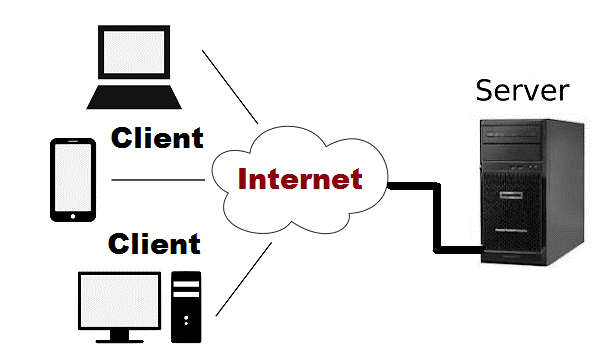
\includegraphics[width=0.5\textwidth]{clientserver}
    \end{center}

    Serverseitiger Code wird zum Beispiel dazu verwendet, einen Nutzer zu \textit{authentifizieren} ("anzumelden"),
    mit Datenbanken zu kommunizieren oder E-Mails zu versenden.
    Damit werden wir uns hier aus Zeitgründen nicht beschäftigen. \\

    Clientseitiger Code auf einer Webseite ist oft dazu da, mit Benutzereingaben oder Hardware zu
    interagieren (Maus, Tastatur, \dots) oder die Webseite dynamisch zu manipulieren (verändern).


    \section{Javascript / Typescript}

    \textit{Javascript} ist eine Programmiersprache die sich als de-facto Standard für clientseitige Programme auf Webseiten
    etabliert hat.
    (Quasi) Jeder Browser kann Javascript sofort ohne Weiteres ausführen.
    Allerdings ist Javascript leider eine schlechte Programmiersprache.
    Ohne darauf näher einzugehen, wollen wir uns stattdessen mit \textit{Typescript} beschäftigen.
    Typescript ist eine Programmiersprache ohne die Schattenseiten von Javascript.
    (Allerdings wird Typescriptcode, den wir schreiben, zu Javascript \textit{transpiliert} (also übersetzt), und das
    übersetzte Javascript wird im Browser ausgeführt).


    \section{Erste Schritte mit Typescript}

    Bevor wir Typescript verwenden können, müssen wir einige Vorbereitungen treffen.
    Uns interessiert in erster Linie das Programmieren an sich, daher müssen die folgenden Schritte zunächst
    nicht zu 100 Prozent verstanden (aber dennoch gemacht) werden.

    \subsection{Mit der Konsole vertraut machen}

    Nicht selten beim Programmieren muss man mit der sogenannten Kommandozeile interagieren.
    Das ist eine alternative Art und Weise den Computer zu steuern, statt mit der Maus Knöpfe zu Klicken
    können wir Befehle eingeben.
    Wir wollen uns nun sehr oberflächlich mit der Kommandozeile befassen.

    Die Windows Kommandozeile heißt \textit{Powershell}.
    Wir geben "Powershell" in die Windows-Suche ein und klicken auf das Ergebnis: \\

    
\includegraphics[width=0.3\textwidth]{powershell}

    Wir sollten etwas sehen, was ungefähr so aussieht: \\

    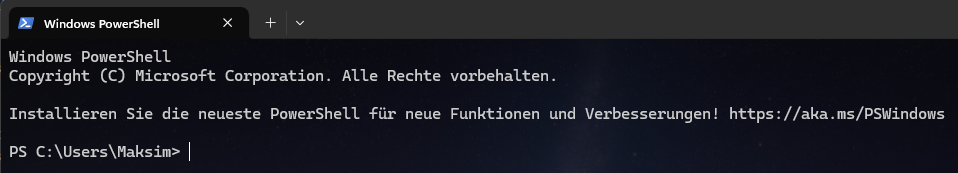
\includegraphics[width=0.8\textwidth]{powershell2}

    In der letzten Zeile links sehen wir das Arbeitsverzeichnis, dort "sind wir gerade", im Bild ist das
    das Verzeichnis \Verb"C:\Users\Maksim".

    Mit dem \Verb"ls"-Befehl können wir uns anzeigen lassen, welche Dateien im aktuellen Verzeichnis sind.
    Geben wir \Verb"ls" ein und drücken Enter, sehen wir eine Liste der Dateien. \\

    \Verb"ll" ist ein Befehl, der keine Argumente (oder Parameter) braucht - es tut immer das Gleiche.
    Andere Befehle brauchen von uns mehr Informationen.
    Hat ein Befehl Argumente, schreiben wir diese einfach dahinter, also in der Form \Verb"Befehl Argument".

    Mit dem Befehl \Verb"cd" können wir das Verzeichnis wechseln.
    Dieser Befehl braucht ein Argument, nämlich die Angabe zu welchem Verzeichnis wir wechseln wollen: \Verb"cd <Ziel>".

    Das Ziel geben wir entweder \textit{relativ} oder \textit{absolut} an.
    \begin{itemize}
        \item Relativ bedeutet: \Verb"cd ziel-ordner" navigiert zu \Verb"<aktueller-ordner>/ziel-ordner".
        \item Absolut bedeutet wir geben den gesamten Pfad zum Zielverzeichnis an, \\
              z.B. \Verb"cd C:\Users\Benutzer\Documents\Ordner1\Ordner2".
    \end{itemize}

    \subsection{Node installieren}

    Zunächst öffnen wir die Kommandozeile und führen den Befehl \Verb"node" aus.
    Sehen wir \textbf{nicht} "\color{red}{... : Die Benennung ... wurde nicht als Name eines Cmdlet,
        einer Funktion, einer Skriptdatei oder eines ausführbaren Programms erkannt.}" so ist node bereits
    installiert und wir können diesen Schritt überspringen.

    Der übliche Weg, mit Typescript zu arbeiten ist über den sogenannten Paketmanager \textit{npm},
    welcher im größeren Softwarepaket \textit{node} enthalten ist.

    Node kann über diese Webseite heruntergeladen und anschließend installiert werden: \url{https://nodejs.org/en}

    Wir verifizieren, dass node korrekt installiert ist, indem wir den Befehl \Verb"node" in die Kommandozeile ausführen
    und sicherstellen, dass es keine Fehlermeldung gibt.
    Auch der Befehl \Verb"npm" sollte keine Fehlermeldung ausgeben.

    \subsection{Typescript im Projekt einrichten}

    Zunächst navigieren wir in der Kommandozeile in den Ordner, in dem unsere Projektdateien liegen.
    Haben wir unsere Dateien zum Beispiel in einem Ordner \Verb"Informatik" auf dem Desktop, führen wir \\
    \Verb"cd C:\Users\<unser nutzer>\Desktop\Informatik" aus (und danach \Verb"ll" um sicherzustellen dass wir im
    richtigen Ordner gelandet sind).

    Jetzt fügen wir das Typescript-Paket zum Projekt hinzu: \Verb"npm install typescript@latest".
    Wenn wir jetzt nochmal \Verb"ll" ausführen (oder einfach über die Windows Oberfläche in den Ordner schauen)
    stellen wir fest, dass zwei neue Dateien erstellt wurden: \Verb"package.json" und \Verb"package-lock.json".
    Dort ist festgehalten, welche Version von Typescript wir verwenden wollen.
    Außerdem wurde der Ordner \Verb"node_modules" erstellt, welcher das Paket Typescript an sich enthält. \\

    Wir müssen nur noch eine Konfigurationsdatei erstellen.
    In unserem Editor (zum Beispiel notepad++) tippen wir folgende Zeilen ein (Groß-Kleinschreibung beachten!):

    \begin{verbatim}
{
   "compilerOptions": {
       "target": "ESNext",
       "module": "ESNext",
       "outDir": "./dist",
       "strict": true,
   }
}
    \end{verbatim}

    Diese Datei speichern wir in unserem Projektordner unter dem Namen \Verb"tsconfig.json".

    \subsection{Erstes Typescript Programm schreiben}

    Wir erstellen eine neue Datei, speichern diese im Projektordner als \Verb"tutorial.ts".
    Hier können wir jetzt unseren Typescript-Code schreiben. \\

    Normale (imperative) Programme (HTML ist kein Programm) bestehen aus Anweisungen,
    die nacheinander ausgeführt werden.

    Wir wollen zum ausprobieren die Anweisung \Verb"alert" ausprobieren.
    Diese ist in der Realität ziemlich nutzlos, aber zum testen ganz witzig.
    Wir schreiben einfach den folgenden Befehl in die erste Zeile unseres noch leeren Programms:

    \begin{verbatim}
        alert("Hallo Welt!")
    \end{verbatim}

    Wie oben beschrieben, muss Typescript-Code vor der ausführung transpiliert werden.
    Das erledigt das Tool \textit{tsc} für uns.
    In der Kommandozeile geben wir ein: \Verb"npx tsc".
    Das Resultat ist ein neuer Ordner \Verb"dist", in dem eine Datei namens \Verb"tutorial.js" liegt
    (man beachte die Dateieendung).

    Um dieses skript nun im Browser ausführen zu lassen, müssen wir es in die Webseite "einbinden".
    Das tun wir im \Verb"<head>" unserer \Verb"index.html" wie folgt:

    \begin{verbatim}
        <head>
            <script type="module" src="./dist/tutorial.js"/>
        </head>
    \end{verbatim}

    Wenn alles richtig funktioniert hat, sollten wir, wenn wir speichern und die Seite im Browser neu laden, etwas zu
    sehen bekommen\dots

    \subsection{Die Browserkonsole}

    Der Browser hat ebenfalls eine eigene Kommandozeile.
    Wir werden diese zu Beginn nutzen, um zu sehen "was unser Typescript-Programm tut" - wir können nämlich
    Dinge auf der Konsole "ausgeben".
    Das tun wir mit folgendem Befehl:

    \begin{verbatim}
        console.log("irgendein text")
        console.log(12345)
        console.log(sonstwas)
    \end{verbatim}


    \subsection{Variablen}

    In den meisten Programmiersprachen gibt es das Konzept von "Variablen".
    Variablen könnten aus dem Mathematikunterricht bekannt sein - gemeint sind meistens "Platzhalter" für irgendetwas.
    So ist das auch beim Programmieren, wir können verschiedene Daten in Variablen speichern und an anderer Stelle
    wieder verwenden.

    In Mathe arbeiten wir meistens mit Zahlen, wenn an der Tafel steht \Verb"x + y" gehen die meisten davon aus
    dass mit \Verb"x" und \Verb"y" irgendwelche Zahlen gemeint sind.
    In einem Programm arbeiten wir meistens mit mehr Dingen als nur Zahlen.

    Daher gibt es das Konzept von "Datentypen", wir definieren welche Art von Daten eine Variable speichern kann.
    In typescript erreichen wir das allgemein wie folgt:

    \begin{verbatim}
        let variablenName: typ
    \end{verbatim}

    Die ersten Datentypen die wir uns anschauen wollen sind \Verb"number" und \Verb"string".
    Wofür \Verb"number" steht ist hoffentlich klar - Zahlen.
    Ein \Verb"string" ist eine Zeichenkette, also eine aneinanderreihung von buchstaben / zahlen / anderen Symbolen.

    Wir könnten also eine Zahl wie folgt definieren:

    \begin{verbatim}
        let warenkorbPreis: number
    \end{verbatim}

    Diese variable hat allerdings noch keinen Wert.
    Den Wert können wir nachträglich ändern:

    \begin{verbatim}
        warenkorbPreis = 370.50
    \end{verbatim}

    Probieren wir mal zusätzlich \Verb"console.log(warenkorbPreis)" in der nächsten Zeile aus. \\

    Wichtig: Wenn wir unseren Typescript code ändern und das Resultat sehen wollen, müssen wir neu transpilieren.
    Also gehen wir wieder in die Windows-Kommandozeile und führen \Verb"npx tsc" aus.

    Laden wir nun unsere Seite im Browser neu, drücken \Verb"F12" und klicken auf
    den Tab "Konsole" (oder "Console") - wir sollten wir unsere eingegebene Zahl sehen.

    Wir können Definition (eigentlich \textit{Deklaration}) und "das Setzen des Wertes" (\textit{Initialisierung})
    auch zusammenfassen:

    \begin{verbatim}
        let warenkorbPreis: number = 370.50
    \end{verbatim}

    Zeichenketten schreiben wir in Typescript stets in Anführungszeichen: \Verb"''das ist ein String''".
    Eine Zeichenkette können wir nicht einer Variable vom Typ \Verb"number" zuweisen.
    Versuchen wir es trotzdem, bekommen wir einen Fehler:

    \begin{verbatim}
        let warenkorbPreis: number
        warenkorbPreis = "banane"
    \end{verbatim}

    Was passiert jetzt, wenn wir \Verb"npx tsc" ausführen? \\

    Strings entsprechen dem Datentyp \Verb"string":

    \begin{verbatim}
        let x: string = "banane"
    \end{verbatim}

    Genauso wie wir Zahlen mit \Verb"+" addieren können (auch in Typescript), können wir Zeichenketten
    addieren:

    \begin{verbatim}
        let links = "mango"
        let rechts = "papaya"
        let summe = links + rechts
    \end{verbatim}

    Was sehen wir, wenn wir summe auf der Konsole ausgeben?
\end{document}
